Motivated by the problems highlighted in the previous section, we propose a new vision of data integration.

%In this scenario, depending on the amount of services available to Marcel, many service compositions could be produced to answer Marcel's query. AA large quantity of
%algorithms for this purpose have been developed, and all of them share the same
%problems: (1) producing rewritings when a big amount of services are available
%is extremely expensive; and (2) not always the quality of the rewriting (composition) produced is enough for meeting your needs.
%Motivated by these problems, our approach proposes a new vision of data
%integration as follows.

Assuming the medical scenario and Marcel's interest in the type of people suffering of a particular disease as before. However, in this new context, he is also capable to express his preferences while integrating services. For instance, he needs to query the patients' personal information and patients' DNA information from patients that were infected by flu, using services with availability higher than 98\%, price per call less than 0.2\$ and total cost less than 2\$. 
Marcel has at his disposal a set of services \textbf{S1}, \textbf{S2}, \textbf{S3} and \textbf{S4} geographically disposed on different cloud provides (configuring a multi-cloud environment).
To achieve his needs, Marcel can use the data services as before invoking in sequence the service \textbf{S1}, \textbf{S3} and \textbf{S4}. However, in this new context, the service selection and rewriting process should meet the user' requirements.   

%This vision of data integration brings some reflections and questions considering the challenges presented previously, such as: (i) The amount of services involved in a multi-cloud context is bigger than in a single cloud. Consequently, the number of services that can be used in the rewriting process and the number of rewriting produced is higher. Such environment calls for a better services selection process, \textit{i.e.}, guided by the SLAs and user preferences; (ii) How can the different SLAs associated to services and cloud provider can be integrated with the user preferences? There are different levels of SLAs: the one agreed between services and cloud providers; and the ones agreed between services and users. These SLAs should be integrated; and (iii) How can a previous processed query be reused for a next query?

%Assuming the same medical scenario and the same families of data services.
%Let us suppose Marcel would like to study the type of people suffering of a
%particular disease as before. However, in this new scenario, he is also capable
%to express his preferences while integrating services. For instance, he needs to
%query the patients' personal information and patients' dna information from
%patients that were infected by flu, using services with availability higher than
%98\%, price per call less than 0.2\$ and total cost less than 2\$. Marcel has at his disposal a set of services from the families \textbf{A}, \textbf{B}, \textbf{C} and \textbf{D} geographically disposed on different cloud provides (configuring a multi-cloud environment).
%To achieve his needs, Marcel can use the data services as before invoking one
%service from the families \textbf{A}, \textbf{C} and \textbf{D} in sequence.
%However, in this new configuration all the services involved must satisfy the
%user preferences expressed in the query. The selection and rewriting process is
%guided by the service level agreements (SLA) exported from different services.
%The user preferences are matched with the service quality aspects that are
%defined on its SLAs.     
%
%This vision of data integration brings some reflections and questions
%considering the challenges presented previously, such as:
%(i) The amount of services involved in a multi-cloud context is bigger than in a
%single cloud. Consequently, the number of services that can be used in the
%rewriting process and the number of rewriting produced is higher. Such
%environment calls for a better services selection process, \textit{i.e.}, guided
%by the SLAs and user preferences; (ii) How can the different SLAs associated to
%services and cloud provider can be integrated with the user preferences? There
%are different levels of SLAs: the one agreed between services and cloud
%providers; and the ones agreed between services and users. These SLAs should be
%integrated; and (iii) How can a previous processed query be reused for a next query?

% Here, it is important to highlight that this paper focus on the description and
% evaluation of the algorithm that rewrites queries in terms of services
% composition taking into account user preferences and service quality aspects
% expressed in SLA contracts. We are assuming that the extraction of quality
% aspects from SLAs is performed in a previous phase of our global data integration solution.
%In the next section we are going to discuss the related works concerning data
%integration and service level agreements, in order to identify the gap between
%the presented challenges and how the works address these problems.

%In recent years, the cloud have been the most popular deployment environment for data integration~\cite{Carvalho2015}. Existing works addressing this issue can be grouped according to two different lines of research:
%\textit{(i)} data integration and services~\cite{Correndo2010,ElSheikh2013,Tian2010,YauY08}; and
%\textit{(ii)} service level agreements (SLA) and data integration~\cite{Bennani2014,Nie07}. 
%
%\cite{Correndo2010} proposed a query rewriting method for achieving RDF data integration. % using SPARQL. The principle of the approach is to rewrite the RDF graph pattern of the query using data manipulation functions in order to: (i) solve the entity co-reference problem which can lead to ineffective data integration; and (ii) exploit ontology alignments with a particular interest in data manipulation. 
%The objective of the approach is to: (i) solve the entity co-reference problem which can lead to ineffective data integration; and (ii) exploit ontology alignments with a particular interest in data manipulation. 
%\cite{ElSheikh2013} introduced a system (called SODIM) which combines data integration, service-oriented architecture and distributed processing. %SODIM works on a pool of collaborative services and can process a large number of databases represented as web services. 
%The novelty of these approaches is that they perform data integration in service oriented contexts, particularly considering data services. They also take into consideration the requirement of computing resources for integrating data. Thus, they exploit parallel settings for implementation costly data integration processes. 
%
%A major concern when integrating data from different sources (services) is privacy that can be associated to the conditions in which integrated data collections are built and shared.
%\cite{YauY08} focused on data privacy based on  a privacy preserving repository in order to integrate data. 
%Based on users' integration requirements, the repository supports the retrieval and integration of
%data across different services. 
%\cite{Tian2010} proposes an inter-cloud data integration system that considers a trade-off between users' privacy requirements and the cost for protecting and processing data. According to the users' privacy requirements, the query plan in the cloud repository creates the users' query. This query is subdivided into sub-queries that can
%be executed in service providers or on a cloud repository. Each option has its own  privacy and processing costs.
%Thus, the query plan executor decides the best location to execute the sub-query to meet privacy and cost constraints.
%
%Service level agreement (SLA) contracts have been widely adopted in the context of Cloud computing. Research contributions mainly concern (i) SLA negotiation phase (step in which the contracts are established between customers and providers) and (ii) monitoring and allocation of cloud resources to detect and avoid SLA violations.
%\cite{Nie07} proposed a data integration model guided by SLAs in a grid environment. Their architecture is subdivided into four parts: (i) a SLA-based resource description model describes the database resources; (ii) a SLA-based query model normalizes the different queries based on the SLA; (iii) a SLA-based matching algorithm selects the databases; and finally (iv) a SLA-based evaluation model obtains the final query solution.
%Apart from our previous work~\cite{Bennani2014}, to the best of our knowledge, there is no evidence of researches on SLA applied to data integration in a (multi-)cloud context.

%\section{SLA guided data integration}
%Given a user query, a set of user preferences associated to it, cloud providers and services, our SLA guided data integration process can be divided in four steps. %The figure 1 illustrates our data integration approach.
%
%\begin{figure}[h!]
%\center
%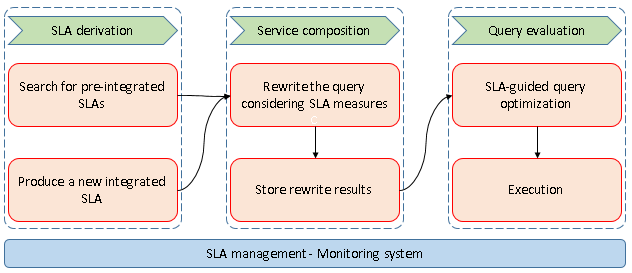
\includegraphics[scale=0.7]{general_approach.PNG}\label{fig:approach}
%\caption{SLA-guided data integration approach}
%\end{figure}

%\underline{The first phase} is the SLA derivation in which a SLA for the user request is created. It consists in looking for a (stored, integrated) SLA derived for a similar request. If a similar SLA is found, the request is forwarded to the query evaluation phase. Otherwise, a new SLA to the integration (called integrated SLA) is produced. The query is expressed as a service composition with associated user preferences. In \underline{the second phase}, service composition, the query is rewritten in terms of different services considering the user preferences and the SLAs of each service involved in the composition. The rewriting result is stored for further uses. \underline{Finally}, in the query evaluation phase, the query is optimized in terms of user preferences and SLAs concerning the consumed resources and the economic cost of the query. Once optimized, the query processed in the execution engine. In addition, we are assuming a SLA management module and monitoring system responsible to verify if the SLA contracts are being respected. Firstly, we have worked on the phases two in order to have an algorithm that will allow us to run important experiments to evaluate our approach. 
Thus, given a user query, a set of user preferences associated to it, cloud providers and services, our SLA guided data integration process can be divided in four steps.
\bigskip

\noindent \underline{SLA derivation}. This step creates an \textsl{integrated SLA} that includes a set of measures corresponding to the user preferences. The \textsl{integrated SLA} guides the query evaluation, and the way results are computed and delivered. \\
\underline{Filtering data services}. The \textsl{integrated SLA} is used (i) to filter previous SLA derived for a similar request in order to reuse previous results; or (ii) to filter possible data services that can be used for answering the query. \\
\underline{Query rewriting}. Given a set of data services that can potentially provide data for integrating the query result, a set of service compositions is generated according to the \textsl{integrated SLA} and the agreed SLA of each data service. \\
\underline{Integrating a query result}. The service compositions are executed in one or several clouds where the user has a subscription. The execution cost of service compositions must fulfill the \textsl{integrated SLA} (that expresses user requirements). Here, the clouds resources needed to execute the composition and how to use them is decided taking in consideration the economic cost determined by the data to be transferred, the number of external calls to services, data storage and delivery cost.
\bigskip

Although \textit{the SLA derivation} is the big challenge while dealing with SLAs and particularly for adding quality dimensions to data integration, the focus in this paper is our query rewriting algorithm which deals with user preferences and SLAs exported by different cloud providers and data services. Here, we are assuming that there is a mechanism responsible to extract the services' quality aspects from SLA, and to provide this information as input to the algorithm. The figure~\ref{fig:cloudsla} illustrates the structure of SLA and its measures that are used inside our approach.

%The first phase is an open issue for dealing with SLAs and particularly for adding quality dimensions to  data integration. The problem is complex because SLA describe different elements participating in the data integration process: data services, cloud services at the different levels of the architecture (i.e., IaaS, PaaS, SaaS), data consumers subscriptions to cloud providers. The SLAs contain measures related to the way services are provided but also related to the data they provide. All these aspects must be considered for matching resources (i.e., services) with data consumers preferences. As shown in the following section and in our study SLA models and languages have been proposed. In contrast  efficient preferences and SLAs matching algorithms need to be proposed to compute derived SLAs. Concerning the other data integration phases, they have been partially addressed by existing works, where some quality dimensions are considered (e.g., data privacy). In our vision there are open issues to be addressed in order to have solutions that consider SLA in order to enhance data integration in multi-cloud environments. 

\begin{figure}[h!]
\center
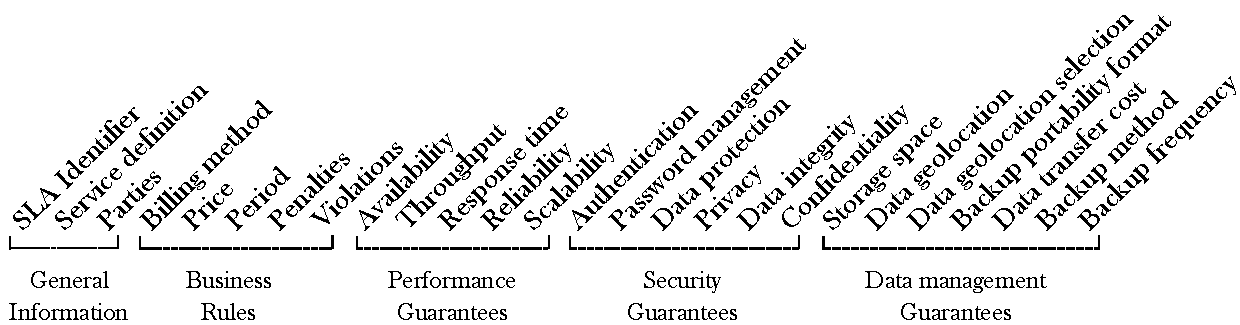
\includegraphics[scale=0.57]{Cloud_SLA.pdf}
\caption{Cloud SLA}\label{fig:cloudsla}
\end{figure}